\documentclass{article}
\usepackage[final]{neurips_2024}
% neurips_2024.sty loads natbib and hyperref itself
\usepackage[utf8]{inputenc}
\usepackage[T1]{fontenc}
\usepackage{url}
\usepackage{booktabs}
\usepackage{amsmath,amssymb}
\usepackage{graphicx}
\bibliographystyle{plainnat}

\title{When Does Self-Supervision Beat ImageNet? \\ Domain Distance Governs Label-Efficient Pretraining in Medical Imaging}

\author{Yang Xingkai \\
  Student ID: G2610153K \\
  MD6329 --- Deep Learning for Healthcare AI}

\begin{document}

\maketitle

\begin{abstract}
Labelled medical images are scarce because annotation requires clinician time, yet
self-supervised pretraining promises to convert unlabelled scans into useful
representations. It is usually unclear \emph{a priori} whether a team should invest in
in-domain self-supervision or simply reuse ImageNet weights. We study this choice
directly by holding the architecture, optimiser, augmentation budget and evaluation
protocol fixed and varying only the initialisation of a ResNet-18 across four arms ---
random, ImageNet transfer, in-domain SimCLR, and sequential ImageNet$\rightarrow$SimCLR
--- over five label budgets (1--100\%), three seeds and two MedMNIST v2 tasks that differ
in how far they sit from natural images: grayscale paediatric chest radiographs
(PneumoniaMNIST) and RGB dermatoscopy (DermaMNIST). Across 210 supervised runs we find
that the ranking of the two pretraining strategies \emph{inverts} with domain distance.
On chest X-ray at a 1\% budget (47 labelled images) in-domain SimCLR reaches
$0.971$ AUROC against $0.917$ for ImageNet transfer and $0.929$ for random
initialisation, a paired gain of $+0.042$ over scratch ($p=0.011$); ImageNet transfer is
not significantly better than scratch on this task at any budget. On dermatoscopy the
opposite holds: ImageNet transfer leads at every budget and in-domain SimCLR never
separates from scratch. With the full label set every pretraining advantage disappears
($p>0.14$), confirming that these methods buy label efficiency rather than peak accuracy.
An augmentation ablation explains part of the asymmetry: removing colour jitter from the
SimCLR view generator \emph{improves} dermatoscopy ($0.798\rightarrow0.823$) while
degrading radiography ($0.982\rightarrow0.959$), because colour carries diagnostic signal
in pigmented lesions but acts only as an intensity augmentation on grayscale film.
In-domain SimCLR is also the best-calibrated and the most corruption-robust arm, losing
only $0.036$ AUROC under severe additive noise where ImageNet transfer loses $0.275$.
We conclude that the useful question is not ``does self-supervision help?'' but ``how far
is this modality from the pretraining corpus, and does the augmentation family preserve
the diagnostic signal?''
\end{abstract}

\section{Problem Formulation}

\paragraph{The clinical problem.} Supervised deep learning in medical imaging is
bottlenecked by labels, not by images. A hospital PACS accumulates studies continuously,
but turning them into a training set requires expert annotation that competes directly
with clinical service time; for dermatoscopy, ground truth often additionally requires
histopathological confirmation \citep{tschandl2018ham10000}. The consequence is the
regime this paper studies: thousands of unlabelled in-domain images alongside only tens
to hundreds of labelled ones. Lecture~1 framed this as one of the field's defining
constraints, and Lecture~2's case studies (Gulshan 2016, Esteva 2017, Rajpurkar 2017)
are precisely the exceptions that required extraordinary labelling effort
\citep{esteva2017dermatologist,rajpurkar2017chexnet}.

\paragraph{Two competing answers.} Practitioners have two standard ways to exploit
structure learned elsewhere. The first, covered in Lecture~2--3 under transfer learning,
initialises from ImageNet \citep{deng2009imagenet,he2016resnet} and fine-tunes. The
second, covered in Lecture~8 on self-supervised and contrastive learning, pretrains on
the unlabelled in-domain images themselves with an objective such as SimCLR
\citep{chen2020simclr}. Both are routinely reported to help, and both are routinely
reported with a single dataset, which makes the practical question --- \emph{which one
should I spend my compute on?} --- unanswerable from the literature.

\paragraph{Research question and hypotheses.} We ask whether the better pretraining
strategy under label scarcity is determined by the distance between the target modality
and the natural-image corpus, and we test four hypotheses:
\textbf{H1} (scarcity) pretraining of either kind helps most at small label budgets and
its advantage vanishes as labels grow;
\textbf{H2} (domain distance) in-domain SimCLR is favoured on a modality far from natural
images (grayscale radiography) whereas ImageNet transfer is favoured on a modality close
to them (RGB dermatoscopy);
\textbf{H3} (augmentation) the optimal SimCLR augmentation family is modality-specific,
because an augmentation that destroys a diagnostic cue cannot yield an invariance worth
having;
\textbf{H4} (composition) sequential ImageNet$\rightarrow$SimCLR pretraining combines
both sources of structure and improves on either alone in the scarce regime.
Our contribution is not a new architecture but a controlled answer to a decision that
every applied team faces, together with the mechanism behind it.

\paragraph{Use of Software 3.0 in problem formulation.} An AI copilot (Claude) was used
to survey candidate framings and datasets. Its first proposals were the generic
``benchmark SSL versus transfer learning on a medical dataset'', which we rejected as a
re-run of published results with no hypothesis. The framing we kept --- two datasets
chosen to \emph{differ in domain distance}, so that the comparison can invert --- came
from pushing back on that suggestion and asking what result would be informative either
way. The copilot also proposed MIMIC-CXR, which we rejected on feasibility grounds
(PhysioNet credentialing takes weeks), and the augmentation-ablation design of H3, which
we kept and sharpened by predicting the \emph{sign} of the colour-jitter effect per
modality before running it. We treat this as the honest record of AI assistance: useful
for breadth and for naming standard practice, unreliable as a source of a sharp question.

\section{Related Work}

\paragraph{Transfer learning in medical imaging.} ImageNet initialisation is the default
in medical computer vision \citep{esteva2021medicalcv} and underpins the landmark results
discussed in Lecture~2 \citep{esteva2017dermatologist,rajpurkar2017chexnet}.
\citet{raghu2019transfusion} questioned the mechanism: for medical targets, much of the
benefit of ImageNet weights comes from better-conditioned scaling of the early layers
rather than from reusable high-level features, and small purpose-built networks often
match transferred ones given enough labels. Our 100\% column reproduces that observation
and extends it by showing the regime where it fails --- at 1\% labels the initialisation
matters enormously.

\paragraph{Self-supervised representation learning.} SimCLR \citep{chen2020simclr} and
MoCo \citep{he2020moco} learn by making two augmented views of the same image agree,
with the augmentation family defining the invariances learned. Lecture~8 (Contrastive
Learning: SimCLR; Weak Supervision) presents exactly this framework, including the
observation that augmentation choice, not architecture, drives representation quality ---
the claim H3 tests in a medical setting. \citet{azizi2021bigselfsupervised} showed that
large self-supervised models improve dermatology and chest X-ray classification,
particularly when in-domain pretraining follows ImageNet pretraining; our H4 arm is a
small-scale version of that recipe, and our robustness analysis shows a failure mode of
it that accuracy alone hides.

\paragraph{Multimodal and text-supervised pretraining.} ConVIRT
\citep{zhang2022convirt} and GLoRIA \citep{huang2021gloria}, both covered in Lecture~8--9
alongside CLIP \citep{radford2021clip}, exploit paired radiology reports as free
supervision and are the strongest label-efficient methods for chest X-ray. They require
paired text, which MedMNIST does not provide; our image-only setting is the regime a team
faces when reports are inaccessible, and our X-ray result (in-domain contrastive
pretraining being decisively better than ImageNet) is consistent with their premise that
in-domain structure is what matters for radiography.

\paragraph{Benchmarks, calibration and robustness.} MedMNIST v2
\citep{yang2023medmnist} standardises lightweight 2D/3D medical classification and
provides the ResNet-18 reference numbers we sanity-check against; its source datasets are
HAM10000 \citep{tschandl2018ham10000} and the paediatric chest X-ray collection of
\citet{kermany2018identifying}. Because accuracy alone is inadequate for clinical
deployment, we additionally report expected calibration error \citep{guo2017calibration}
and corruption robustness in the style of \citet{hendrycks2019robustness}, both themes of
Lecture~11 (Interpretability, Fairness, Uncertainty, Robustness), and we interpret models
with Grad-CAM \citep{selvaraju2017gradcam}, the attribution method introduced in that
same lecture. Our optimiser follows \citet{loshchilov2019adamw} and our GPU augmentation
uses Kornia \citep{riquelme2025kornia}.

\paragraph{Where this work sits.} Prior work establishes that both pretraining strategies
help, usually one dataset at a time. We hold everything but the initialisation fixed,
evaluate two modalities chosen to differ in domain distance, and report label efficiency,
calibration, robustness and augmentation sensitivity together. The result --- that the
ranking inverts, and that the augmentation that helps one modality hurts the other --- is
a statement about \emph{when} each method applies rather than which is better.

\section{Data}

We use two MedMNIST v2 \citep{yang2023medmnist} tasks at $64\times64$ resolution with the
official train/validation/test splits, which are patient-disjoint in the source datasets.

\textbf{PneumoniaMNIST} derives from paediatric chest radiographs
\citep{kermany2018identifying}: 4{,}708 training, 524 validation and 624 test images,
grayscale, binary (normal versus pneumonia), with 74\% of training images positive.
\textbf{DermaMNIST} derives from HAM10000 \citep{tschandl2018ham10000}: 7{,}007 training,
1{,}003 validation and 2{,}005 test images, RGB, seven lesion classes with severe
imbalance --- melanocytic nevi account for 4{,}693 training images while dermatofibroma
has 80. Figure~\ref{fig:data} shows examples and the full class distribution.

\begin{figure}[t]
\centering
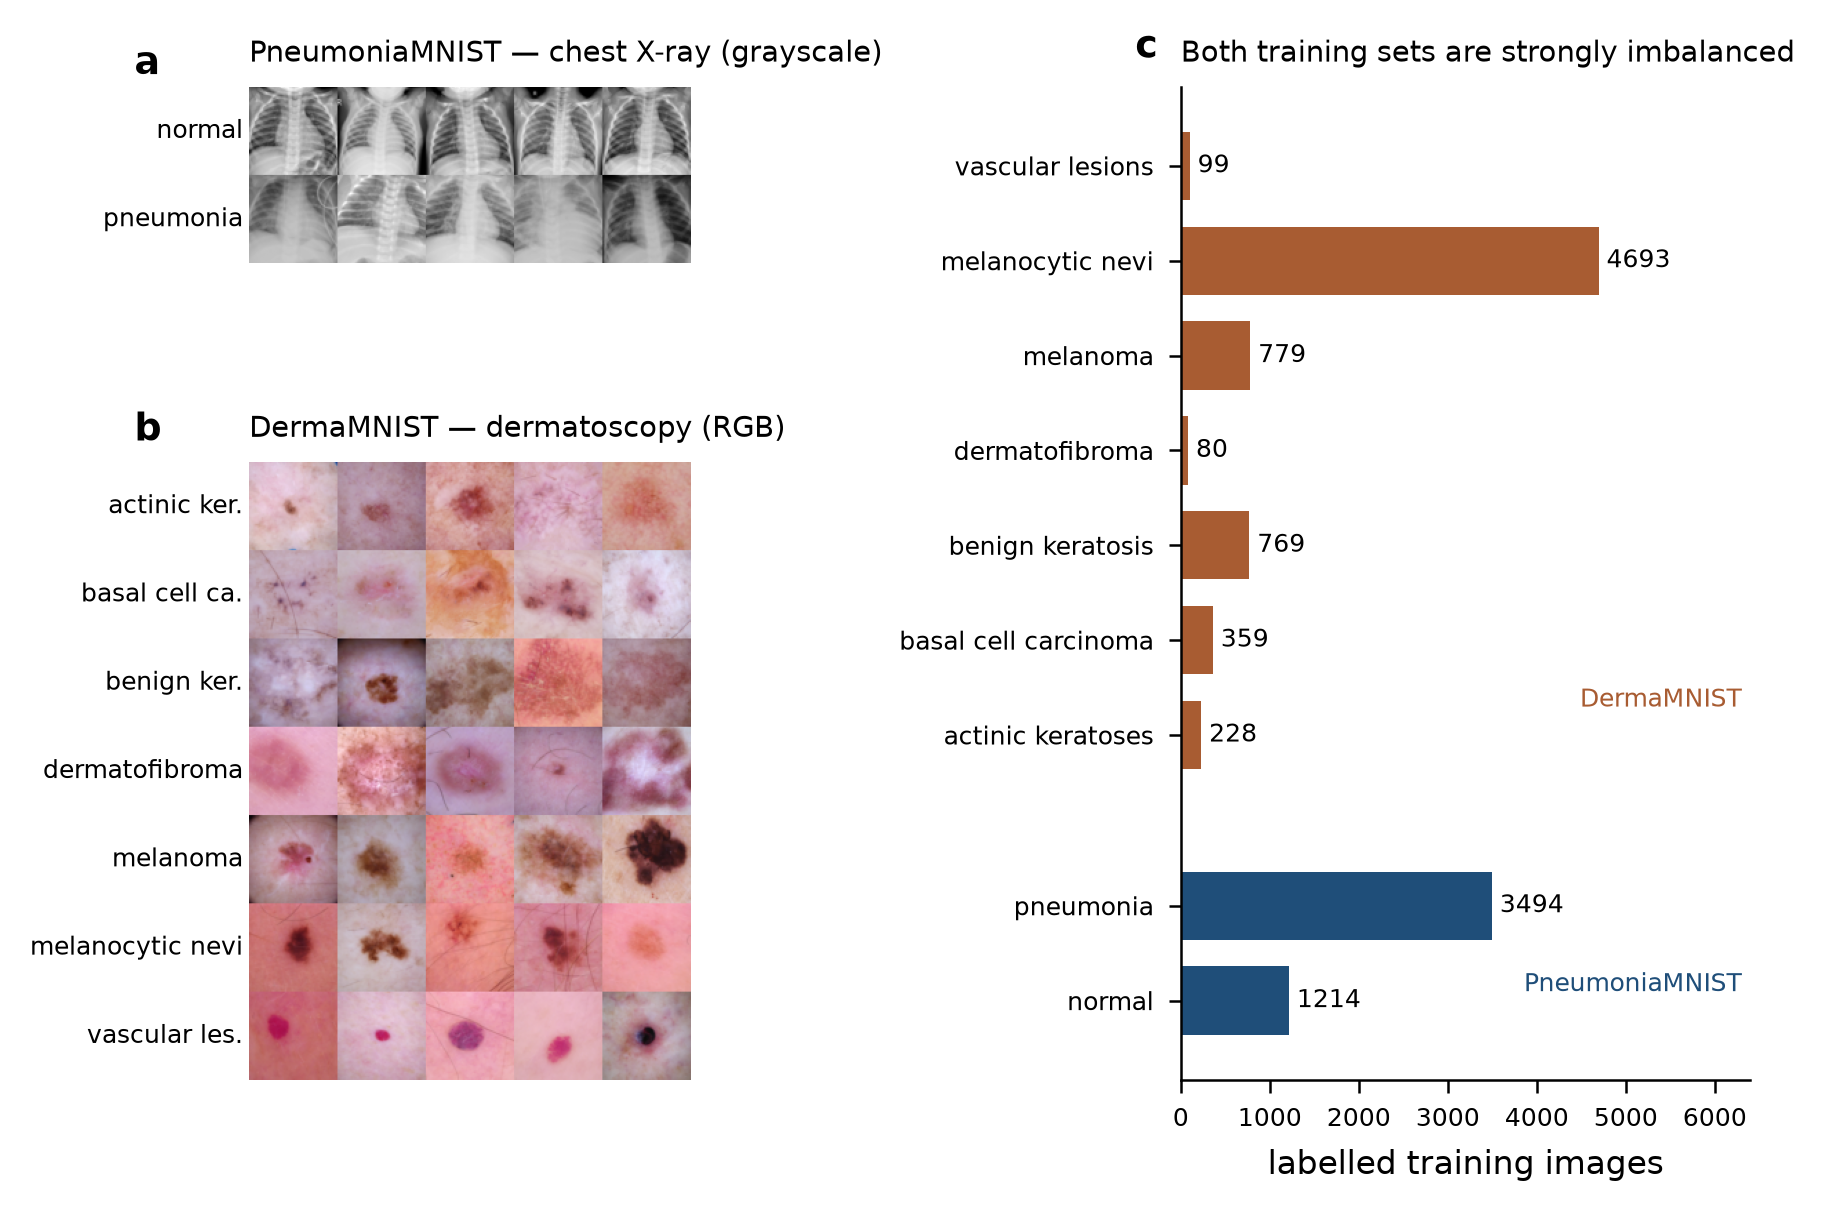
\includegraphics[width=\textwidth]{figs/fig1_data.png}
\caption{The two tasks. (a--b) Five random training examples per class; the modalities
differ in channel statistics, in what constitutes the diagnostic cue (opacity and lung
texture versus lesion pigmentation and border), and in how closely they resemble natural
images. (c) Training-set class counts; both tasks are strongly imbalanced, which is why
every model is trained with a class-weighted loss and evaluated with balanced accuracy
and AUPRC in addition to AUROC.}
\label{fig:data}
\end{figure}

\paragraph{Label budgets.} The label-scarcity axis is created by class-stratified
subsampling of the training split at fractions $\{1,5,10,25,100\}\%$. Subsets are
\emph{nested} within a seed (the 1\% subset is contained in the 5\% subset, verified
programmatically), so differences along the curve reflect the budget rather than which
images happened to be drawn, and every class retains at least five examples so that no
class disappears. The 1\% budget corresponds to 47 labelled chest radiographs and 83
dermatoscopic images --- the latter spread over seven classes, i.e. 5--56 images per
class. Validation and test splits are always complete; only the training labels are
restricted, which mirrors the real situation of having abundant unlabelled data.

\paragraph{Unlabelled data for pretraining.} Self-supervised pretraining uses the images
of the full training split with labels discarded (4{,}708 and 7{,}007 images). This is
deliberately a \emph{small} unlabelled corpus by self-supervised standards and bounds how
much in-domain SimCLR can be expected to achieve.

\paragraph{Preprocessing.} Images are kept at $64\times64$, scaled to $[0,1]$, and
normalised with ImageNet channel statistics in every arm so that normalisation is not a
confound. Grayscale images are replicated to three channels so that one unmodified
architecture serves all arms.

\section{Approach}

\paragraph{Design principle.} The experiment is designed so that the only difference
between arms is the \emph{initialisation} of the backbone. Architecture, input
resolution, normalisation, supervised augmentation, loss, optimiser, schedule, early
stopping and model selection are identical across arms, which is what licenses reading a
difference in test metric as an effect of pretraining.

\paragraph{Backbone.} An unmodified torchvision ResNet-18 \citep{he2016resnet}, including
its $7\times7$/stride-2 stem, fed with $64\times64$ inputs (final feature map
$2\times2$, 512-dimensional pooled embedding). Keeping the ImageNet stem rather than
substituting a CIFAR-style $3\times3$ stem costs some spatial resolution but is the only
way to reuse ImageNet weights without surgery, and therefore the only way to keep the
architecture common to all four arms.

\paragraph{Arms.} (i) \emph{From scratch}: random initialisation. (ii) \emph{ImageNet
transfer}: \texttt{IMAGENET1K\_V1} weights. (iii) \emph{In-domain SimCLR}: SimCLR
pretraining on the unlabelled in-domain images from random initialisation.
(iv) \emph{ImageNet + SimCLR}: the same SimCLR pretraining started from ImageNet weights.

\paragraph{SimCLR pretraining.} Two views per image are drawn from the standard SimCLR
family --- random resized crop (scale $0.2$--$1.0$), horizontal flip, colour jitter
$(0.8,0.8,0.8,0.2)$ with probability $0.8$, random grayscale ($p{=}0.2$) and Gaussian
blur ($5\times5$, $\sigma\in[0.1,2]$, $p{=}0.5$). A two-layer MLP head
($512\rightarrow512\rightarrow128$) projects the pooled features, and the NT-Xent loss
\citep{chen2020simclr} with temperature $\tau=0.5$ treats the other view as the positive
and the remaining $2N-2$ elements of the batch as negatives:
\begin{equation}
\mathcal{L}_{i} = -\log \frac{\exp(\mathrm{sim}(z_i, z_{j(i)})/\tau)}
{\sum_{k \neq i} \exp(\mathrm{sim}(z_i, z_k)/\tau)}, \qquad
\mathrm{sim}(u,v) = \frac{u^\top v}{\lVert u\rVert \lVert v\rVert}.
\end{equation}
We pretrain for 400 epochs with AdamW \citep{loshchilov2019adamw} (learning rate
$10^{-3}$, weight decay $10^{-6}$), batch size 256 and a cosine schedule. The loss is
computed in float32 with autocast disabled, because under mixed precision the
self-similarity mask overflows the float16 range --- a concrete implementation detail
that silently produces NaNs if missed.

\paragraph{Supervised training.} Each labelled subset is trained for at most 40 epochs
with AdamW (learning rate $3\times10^{-4}$ for pretrained initialisations,
$10^{-3}$ for random initialisation and for linear probes; weight decay $10^{-4}$),
batch size $\min(128, \max(8, N/4))$, cosine schedule, and augmentation limited to random
resized crop (scale $0.7$--$1.0$) and horizontal flip. The loss is cross-entropy with
inverse-frequency class weights and label smoothing $0.05$. We select the epoch with the
best \emph{validation} AUROC (patience 8) and evaluate the test split exactly once with
those weights, so no test information enters model selection. Linear probes freeze the
backbone (kept in eval mode so its batch-norm statistics are not updated) and train only
the final linear layer.

\paragraph{Metrics.} We report AUROC and AUPRC (macro one-vs-rest for the seven-class
task), balanced accuracy, macro-averaged sensitivity and specificity, and expected
calibration error with 15 equal-width confidence bins \citep{guo2017calibration}.
Balanced accuracy and AUPRC are emphasised because accuracy is uninformative when 67\% of
dermatoscopy images belong to one class. Every configuration is run with seeds
$\{0,1,2\}$ and we report the mean with a 95\% $t$-interval; comparisons against the
scratch arm use a paired $t$-test over seeds, pairing on the seed that also determines
the label subset.

\paragraph{Implementation and Software 3.0.} PyTorch 2.11 (CUDA 12.8) on one RTX 5090;
both datasets are held resident in GPU memory as tensors and augmented in batch with
Kornia \citep{riquelme2025kornia}, with per-sample augmentation parameters. This was a
necessary engineering decision rather than an optimisation: the execution sandbox denies
named-pipe creation, so multi-process \texttt{DataLoader} workers are unavailable and
in-process CPU augmentation capped throughput at 8--12\,s per pretraining epoch; moving
augmentation onto the device reduced this to 0.8--1.2\,s and made 12 pretraining runs and
210 supervised runs feasible in about two hours. An AI copilot wrote much of the
scaffolding (data module, metric functions, sweep driver) and diagnosed two failures that
cost real time --- the float16 overflow in NT-Xent and an OpenMP runtime clash between a
conda MKL NumPy and the venv PyTorch. It was least reliable where it mattered most: its
initial experiment driver evaluated on the test split for model selection, which we
replaced with validation-based selection. We report this because it is the pattern we
observed throughout --- AI assistance compressed implementation time substantially while
leaving experimental validity entirely to the authors.

\section{Experiments}

All numbers are test-set means over three seeds with 95\% $t$-intervals;
$^{*}$ marks $p<0.05$ in a paired $t$-test against the scratch arm.

\subsection{Label efficiency and the inversion (H1, H2)}

Table~\ref{tab:main} and Figure~\ref{fig:curves} give the main result. Both classical
baselines are beaten by every neural arm on chest X-ray, but on dermatoscopy a pixel
random forest ($0.807$ AUROC at 100\% labels) is a stronger baseline than one might
expect and exceeds every neural arm at the 1\% budget --- a useful reminder that deep
models are not automatically preferable when labels are very scarce.

\begin{table}[t]
\centering
\caption{Test AUROC by initialisation and label budget (mean $\pm$ 95\% CI over three
seeds). The pixel random forest is the non-neural reference.}
\label{tab:main}
\small
\begin{tabular}{llccccc}
\toprule
Dataset & Initialisation & \multicolumn{5}{c}{Labelled fraction of the training set} \\
\cmidrule(lr){3-7}
 & & 1\% & 5\% & 10\% & 25\% & 100\% \\
\midrule
PneumoniaMNIST & pixel random forest & 0.909\,{\tiny $\pm$\,0.022} & 0.931\,{\tiny $\pm$\,0.030} & 0.932\,{\tiny $\pm$\,0.022} & 0.940\,{\tiny $\pm$\,0.012} & 0.944\,{\tiny $\pm$\,0.002} \\
 & from scratch & 0.929\,{\tiny $\pm$\,0.026} & 0.957\,{\tiny $\pm$\,0.027} & 0.936\,{\tiny $\pm$\,0.026} & 0.971\,{\tiny $\pm$\,0.005} & 0.979\,{\tiny $\pm$\,0.016} \\
 & ImageNet transfer & 0.917\,{\tiny $\pm$\,0.020} & 0.953\,{\tiny $\pm$\,0.085} & 0.954\,{\tiny $\pm$\,0.036} & 0.984\,{\tiny $\pm$\,0.013} & 0.985\,{\tiny $\pm$\,0.018} \\
 & in-domain SimCLR & 0.971\,{\tiny $\pm$\,0.028} & 0.983\,{\tiny $\pm$\,0.011} & 0.982\,{\tiny $\pm$\,0.019} & 0.986\,{\tiny $\pm$\,0.016} & 0.985\,{\tiny $\pm$\,0.005} \\
 & ImageNet + SimCLR & 0.980\,{\tiny $\pm$\,0.002} & 0.990\,{\tiny $\pm$\,0.002} & 0.987\,{\tiny $\pm$\,0.006} & 0.994\,{\tiny $\pm$\,0.002} & 0.976\,{\tiny $\pm$\,0.030} \\
\midrule
DermaMNIST & pixel random forest & 0.683\,{\tiny $\pm$\,0.046} & 0.710\,{\tiny $\pm$\,0.011} & 0.744\,{\tiny $\pm$\,0.015} & 0.763\,{\tiny $\pm$\,0.010} & 0.807\,{\tiny $\pm$\,0.004} \\
 & from scratch & 0.754\,{\tiny $\pm$\,0.072} & 0.744\,{\tiny $\pm$\,0.130} & 0.795\,{\tiny $\pm$\,0.015} & 0.843\,{\tiny $\pm$\,0.061} & 0.880\,{\tiny $\pm$\,0.051} \\
 & ImageNet transfer & 0.753\,{\tiny $\pm$\,0.039} & 0.780\,{\tiny $\pm$\,0.027} & 0.823\,{\tiny $\pm$\,0.057} & 0.845\,{\tiny $\pm$\,0.027} & 0.914\,{\tiny $\pm$\,0.049} \\
 & in-domain SimCLR & 0.738\,{\tiny $\pm$\,0.063} & 0.765\,{\tiny $\pm$\,0.039} & 0.798\,{\tiny $\pm$\,0.062} & 0.840\,{\tiny $\pm$\,0.025} & 0.887\,{\tiny $\pm$\,0.030} \\
 & ImageNet + SimCLR & 0.743\,{\tiny $\pm$\,0.042} & 0.773\,{\tiny $\pm$\,0.038} & 0.818\,{\tiny $\pm$\,0.025} & 0.855\,{\tiny $\pm$\,0.043} & 0.891\,{\tiny $\pm$\,0.038} \\
\bottomrule
\end{tabular}
\end{table}

\begin{figure}[t]
\centering
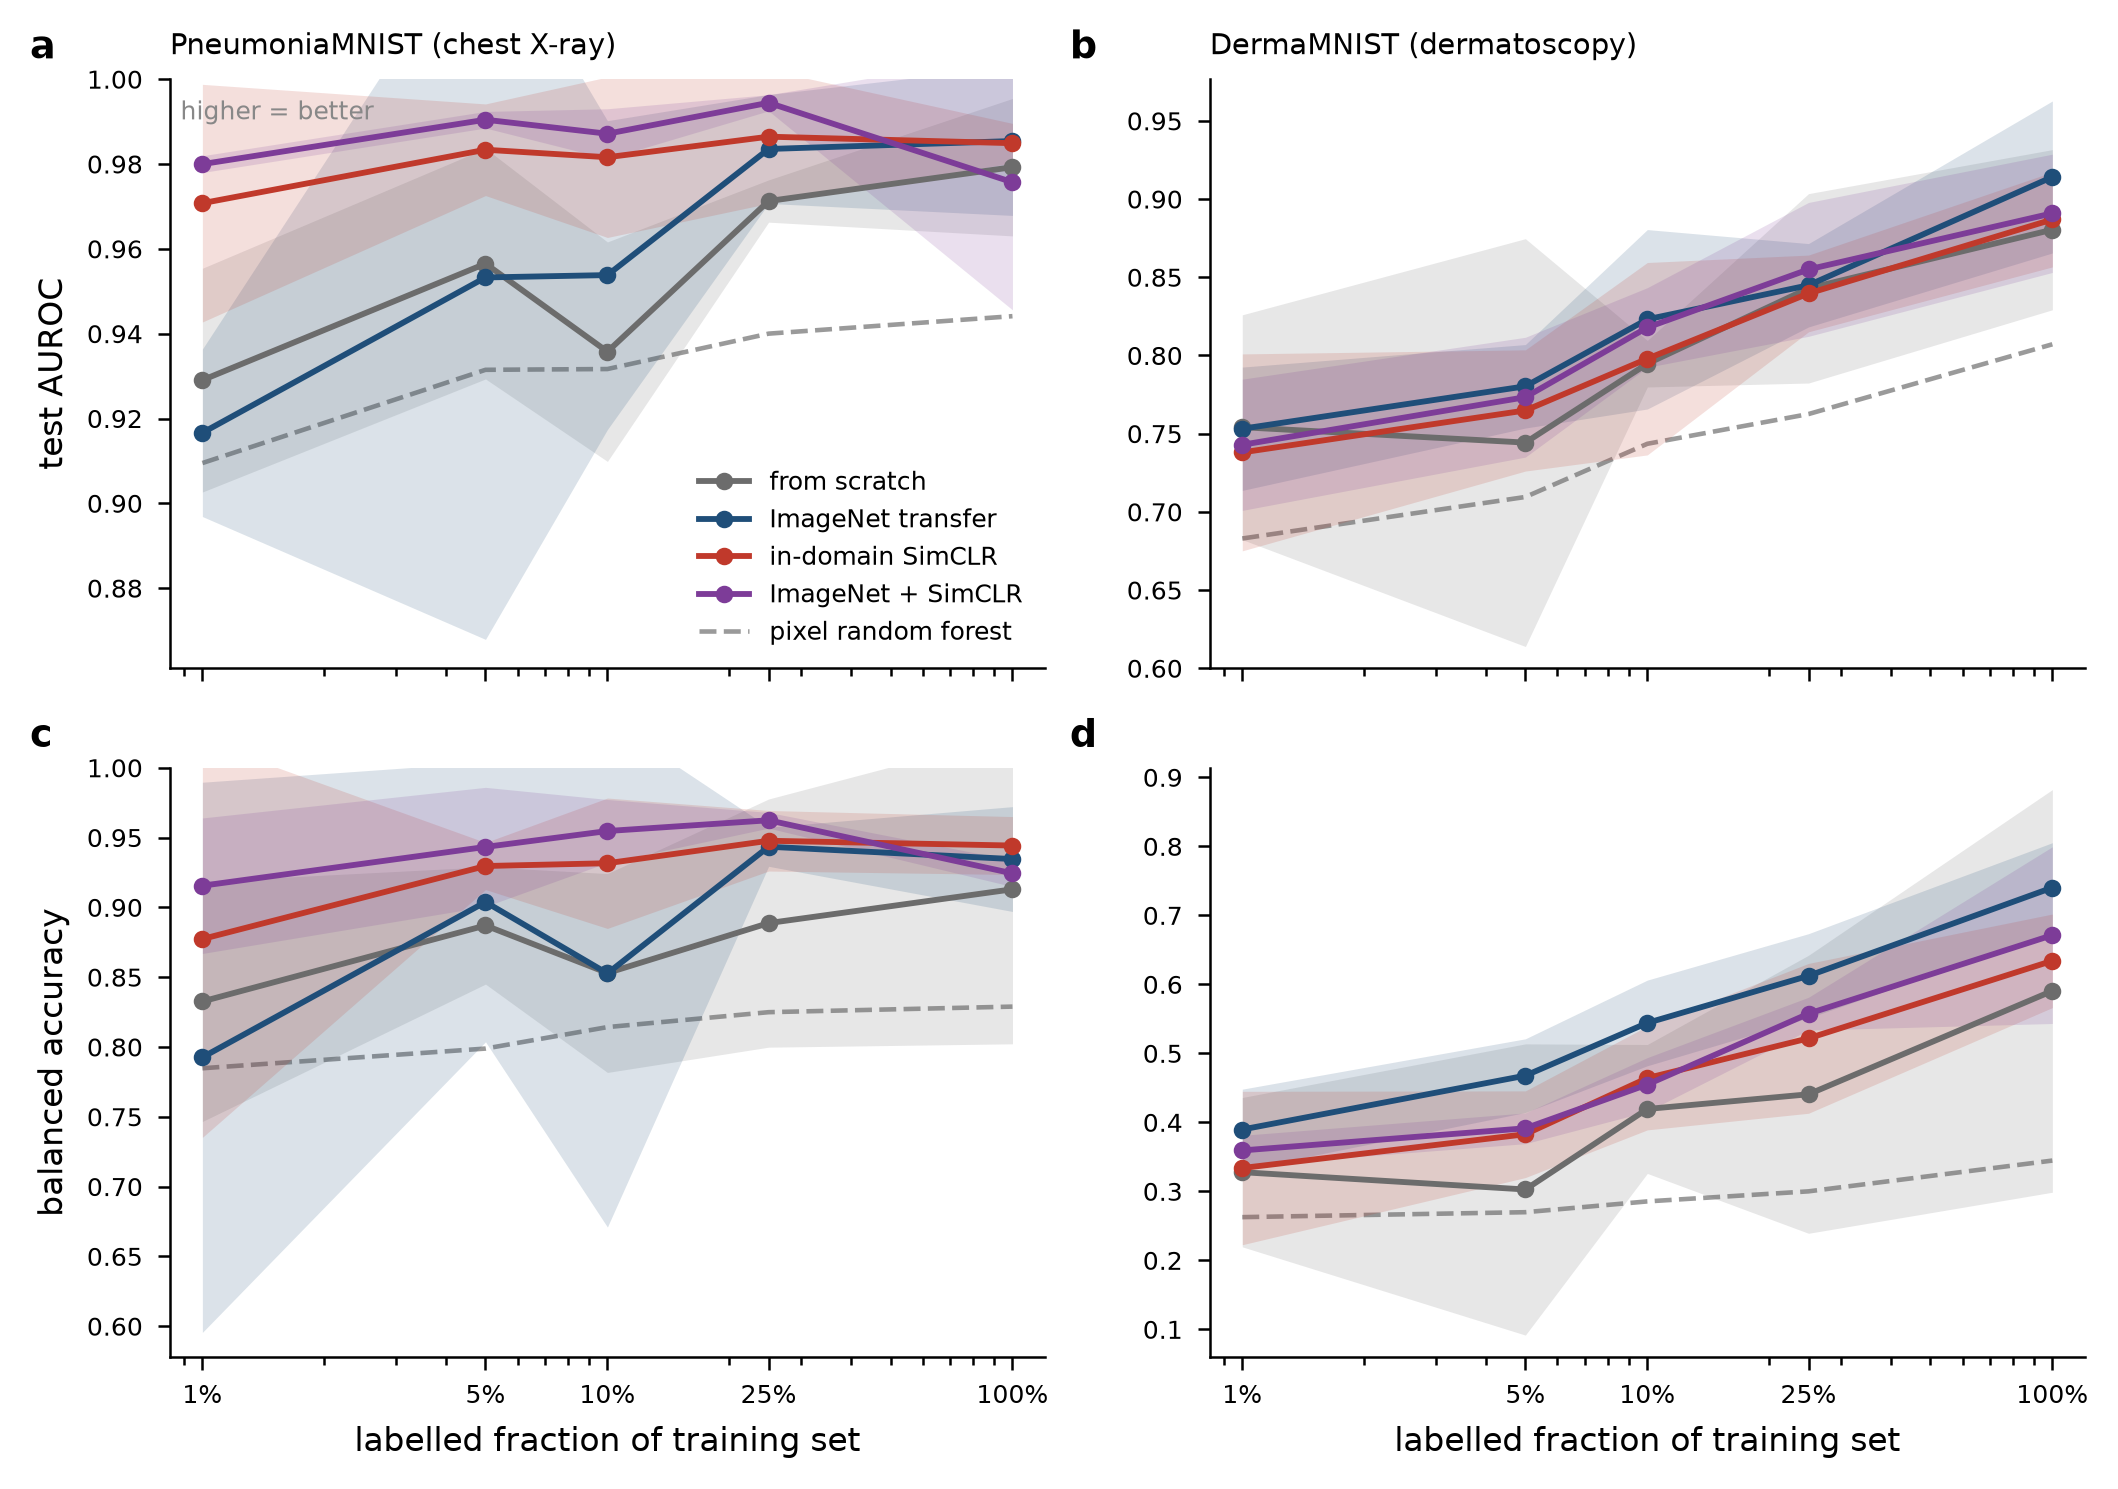
\includegraphics[width=\textwidth]{figs/fig2_label_efficiency.png}
\caption{Label-efficiency curves. (a--b) AUROC and (c--d) balanced accuracy against the
labelled fraction. On chest X-ray the two SimCLR arms dominate from 1\% labels onward and
ImageNet transfer tracks the scratch arm; on dermatoscopy the ordering reverses, with
ImageNet transfer best at every budget in balanced accuracy. Shaded bands are 95\%
$t$-intervals over three seeds; the dashed line is the pixel random forest.}
\label{fig:curves}
\end{figure}

\paragraph{The ranking inverts with domain distance (H2, supported).} On PneumoniaMNIST
at 1\% labels (47 images) in-domain SimCLR reaches $0.971$ AUROC and sequential
ImageNet+SimCLR $0.980$, against $0.917$ for ImageNet transfer and $0.929$ for scratch.
The paired gains over scratch in Table~\ref{tab:deltas} are $+0.042$ ($p=0.011$) and
$+0.051$ ($p=0.012$); ImageNet transfer is \emph{not} significantly better than scratch at
any budget on this task, and is numerically worse at 1\%. On DermaMNIST the pattern
reverses: ImageNet transfer leads at every budget, most visibly in balanced accuracy
($0.544$ versus $0.464$ for in-domain SimCLR at 10\% labels, and $0.740$ versus $0.634$ at
100\%), while in-domain SimCLR never separates from scratch ($+0.003$, $p=0.84$ at 10\%).
The effect we hypothesised is therefore present with the predicted sign in both
directions: in-domain self-supervision wins where the modality is far from natural
images, ImageNet transfer wins where it is close.

\paragraph{Pretraining buys label efficiency, not peak accuracy (H1, supported).}
At the full label budget no arm is significantly better than scratch on either task (all
$p>0.14$; Table~\ref{tab:deltas}). The benefit is concentrated at small budgets, and on
chest X-ray it is large enough that the scratch arm never reaches the SimCLR arms' 10\%
performance at \emph{any} budget we tested, including 100\% labels. This is the
\citet{raghu2019transfusion} observation --- initialisation stops mattering once labels
are plentiful --- with the complementary half made explicit.

\begin{table}[t]
\centering
\caption{Paired difference in test AUROC against the from-scratch arm (same seeds, same
label subsets). $^{*}$: $p<0.05$, paired $t$-test, $n=3$ seeds.}
\label{tab:deltas}
\small
\begin{tabular}{llccc}
\toprule
Dataset & Initialisation & 1\% labels & 10\% labels & 100\% labels \\
\midrule
PneumoniaMNIST & ImageNet transfer & -0.012 & +0.018 & +0.006 \\
 & in-domain SimCLR & +0.042$^{*}$ & +0.046$^{*}$ & +0.006 \\
 & ImageNet + SimCLR & +0.051$^{*}$ & +0.051$^{*}$ & -0.004 \\
\midrule
DermaMNIST & ImageNet transfer & -0.001 & +0.028 & +0.034 \\
 & in-domain SimCLR & -0.016 & +0.003 & +0.007 \\
 & ImageNet + SimCLR & -0.011 & +0.023 & +0.010 \\
\bottomrule
\end{tabular}
\end{table}

\paragraph{Sequential pretraining helps on X-ray only (H4, partially supported).}
ImageNet+SimCLR is the best arm on PneumoniaMNIST at every budget below 100\%, slightly
ahead of in-domain SimCLR, so the two sources of structure do compose where
self-supervision works. On DermaMNIST it lands between the two single-source arms and
does not beat ImageNet transfer. Composition therefore inherits, rather than repairs, the
weakness of its in-domain component; and Section~\ref{sec:robust} shows it also inherits a
brittleness that neither parent exhibits.

\subsection{Linear probes: what the representation already contains}

Table~\ref{tab:probe} separates representation quality from adaptation. On chest X-ray a
\emph{frozen} in-domain SimCLR backbone with a single trained linear layer reaches
$0.989$ AUROC --- better than fine-tuning the same weights ($0.982$) and far better than a
frozen ImageNet backbone ($0.921$). The pneumonia decision is thus close to linearly
decodable from representations learned without a single label, which is the strongest
evidence here that in-domain self-supervision has captured task-relevant structure rather
than merely a good initialisation. On dermatoscopy no frozen representation is adequate
(probes lose to fine-tuning for every arm), consistent with the seven-class fine-grained
task requiring feature adaptation.

\begin{table}[t]
\centering
\caption{Frozen linear probe versus full fine-tuning at the 10\% label budget (test
AUROC). A positive final column means the frozen representation is already better than
what fine-tuning reaches.}
\label{tab:probe}
\small
\begin{tabular}{llccc}
\toprule
Dataset & Initialisation & Fine-tune & Linear probe & Probe $-$ fine-tune \\
\midrule
PneumoniaMNIST & ImageNet transfer & 0.954 & 0.921 & -0.033 \\
 & in-domain SimCLR & 0.982 & 0.989 & +0.007 \\
 & ImageNet + SimCLR & 0.987 & 0.991 & +0.004 \\
\midrule
DermaMNIST & ImageNet transfer & 0.823 & 0.815 & -0.008 \\
 & in-domain SimCLR & 0.798 & 0.776 & -0.022 \\
 & ImageNet + SimCLR & 0.818 & 0.816 & -0.002 \\
\bottomrule
\end{tabular}
\end{table}

\subsection{Which augmentation matters, and why it is modality-specific (H3)}

Table~\ref{tab:ablation} and Figure~\ref{fig:probe}c ablate one component at a time from
the SimCLR view generator, keeping the pretraining budget fixed and fine-tuning at 10\%
labels.

\begin{table}[t]
\centering
\caption{SimCLR augmentation ablation: test AUROC at the 10\% label budget after
pretraining with one component removed (mean $\pm$ 95\% CI, three seeds).}
\label{tab:ablation}
\small
\begin{tabular}{lcc}
\toprule
Pretraining augmentation & PneumoniaMNIST & DermaMNIST \\
\midrule
full SimCLR augmentation & 0.982\,{\tiny $\pm$\,0.019} & 0.798\,{\tiny $\pm$\,0.062} \\
no colour jitter & 0.959\,{\tiny $\pm$\,0.034} & 0.823\,{\tiny $\pm$\,0.022} \\
no random resized crop & 0.921\,{\tiny $\pm$\,0.024} & 0.725\,{\tiny $\pm$\,0.065} \\
no Gaussian blur & 0.981\,{\tiny $\pm$\,0.027} & 0.790\,{\tiny $\pm$\,0.014} \\
no horizontal flip & 0.984\,{\tiny $\pm$\,0.012} & 0.800\,{\tiny $\pm$\,0.032} \\
\bottomrule
\end{tabular}
\end{table}

\begin{figure}[t]
\centering
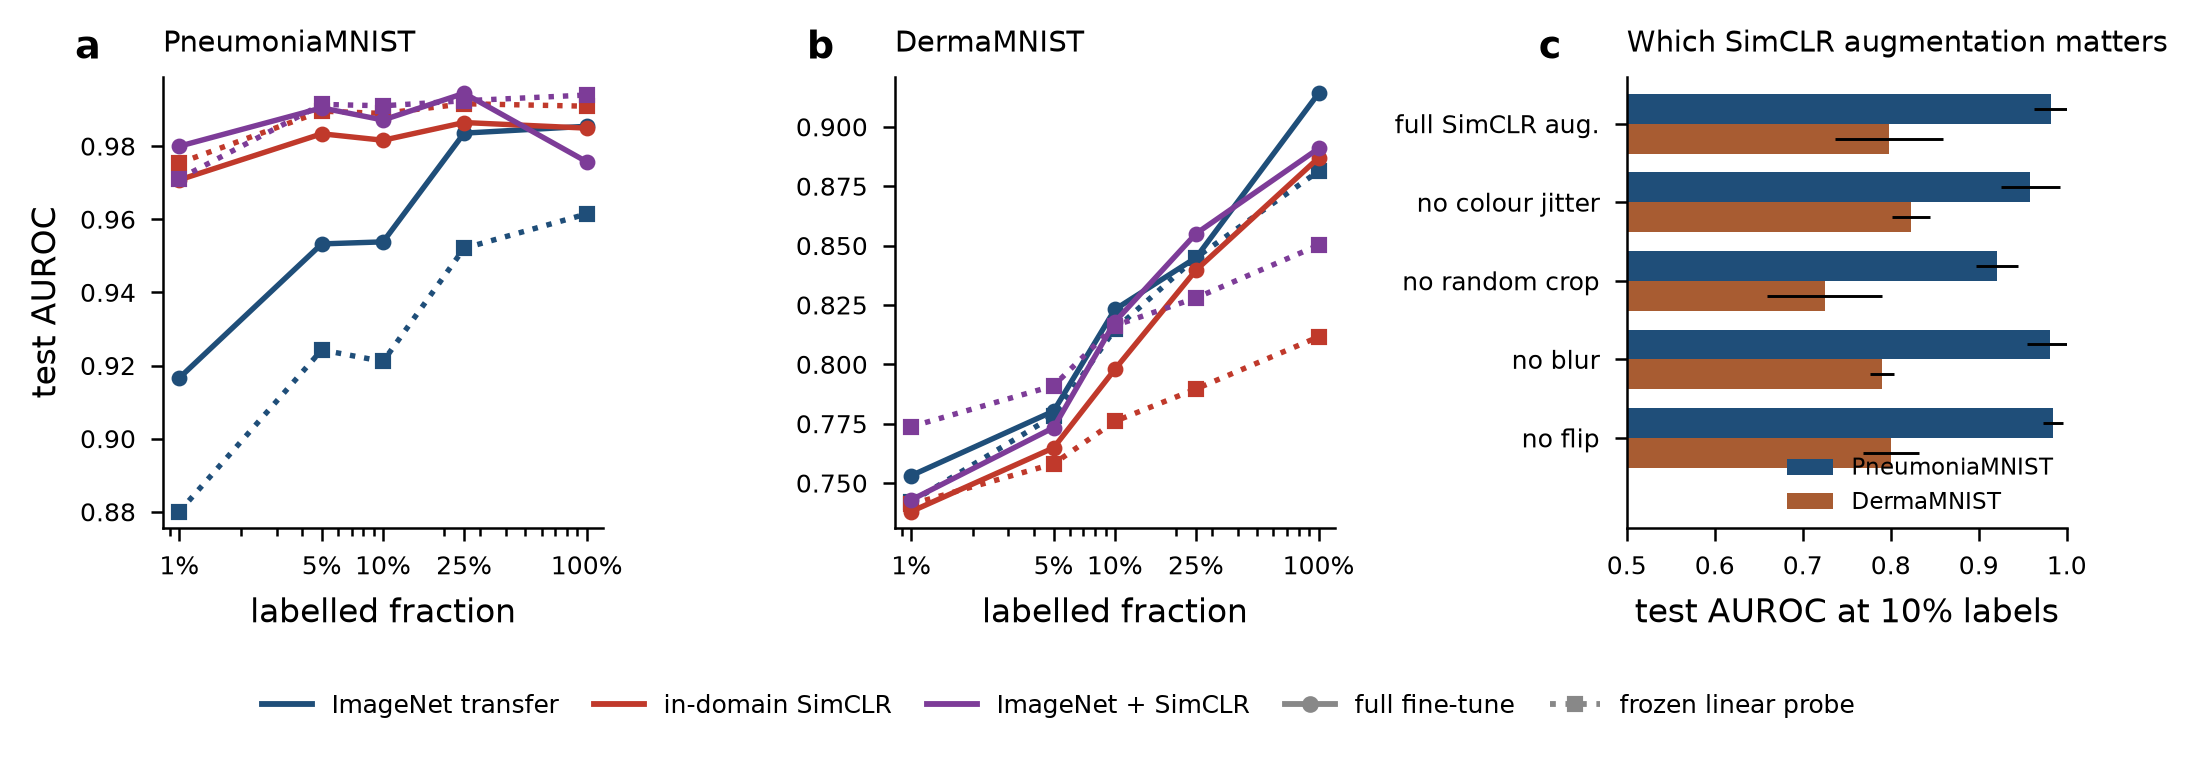
\includegraphics[width=\textwidth]{figs/fig3_probe_ablation.png}
\caption{(a--b) Frozen linear probe (dotted) versus full fine-tuning (solid). The
in-domain SimCLR probe exceeds its own fine-tuned counterpart on chest X-ray, and the
ImageNet probe falls far behind. (c) Augmentation ablation at 10\% labels: random
resized crop is essential on both modalities, whereas removing colour jitter helps
dermatoscopy and hurts radiography.}
\label{fig:probe}
\end{figure}

\paragraph{Random crop is indispensable; colour jitter is not, and its sign flips.}
Removing random resized crop is the single most damaging change on both tasks
($0.982\rightarrow0.921$ on X-ray, $0.798\rightarrow0.725$ on dermatoscopy): without
spatial cropping the contrastive task is too easy and the representation collapses toward
low-level cues. Colour jitter behaves oppositely across modalities. Removing it
\emph{improves} DermaMNIST from $0.798$ to $0.823$ --- the best dermatoscopy SimCLR result
we obtained --- but \emph{degrades} PneumoniaMNIST from $0.982$ to $0.959$. The
interpretation is mechanical and clinically sensible: in pigmented-lesion analysis colour
and its variegation \emph{are} diagnostic criteria, so forcing the encoder to be invariant
to hue and saturation discards the signal the downstream task needs; on single-channel
radiographs the same transform reduces to brightness and contrast perturbation, which
mimics real exposure variation and is useful. H3 is supported, and in the strong form: the
best augmentation family is not a property of SimCLR but of the modality.

\subsection{Calibration, rare classes, robustness and attribution}
\label{sec:robust}

\begin{figure}[t]
\centering
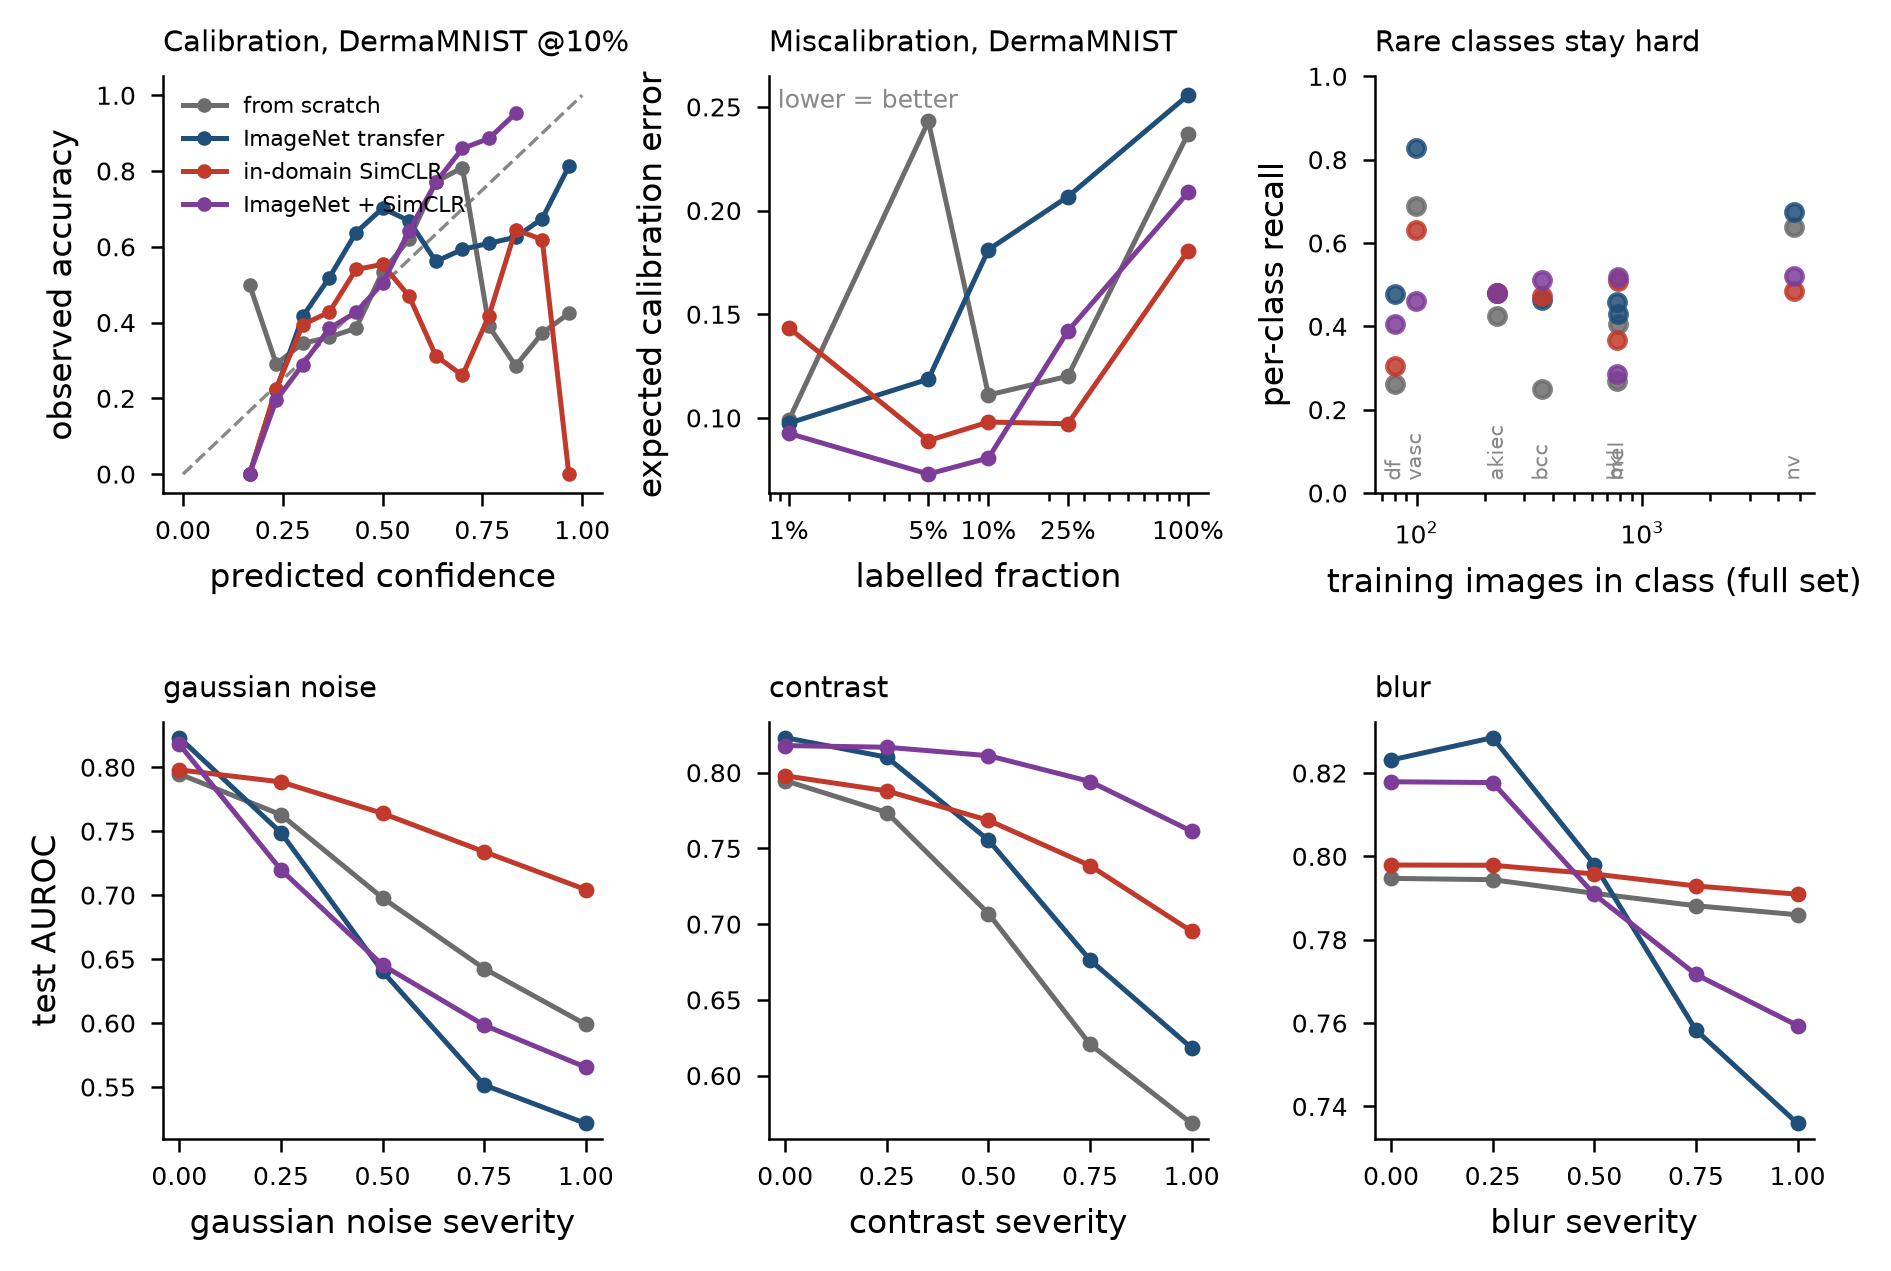
\includegraphics[width=\textwidth]{figs/fig4_analysis.png}
\caption{DermaMNIST analyses. (a) Reliability diagram at 10\% labels. (b) Expected
calibration error against label budget. (c) Per-class recall at 10\% labels against class
frequency in the full training set; the four rarest classes remain poorly detected by
every arm. (d--f) Test-time corruption robustness at the 10\% budget, mean over three
seeds.}
\label{fig:analysis}
\end{figure}

\paragraph{Calibration.} At the 10\% dermatoscopy budget, expected calibration error is
$0.081$ for ImageNet+SimCLR and $0.098$ for in-domain SimCLR, against $0.181$ for ImageNet
transfer and $0.111$ for scratch. The arm with the best discrimination on this task
(ImageNet transfer) is thus the worst calibrated --- its confidences are not usable as
probabilities without recalibration, which matters more than a 0.02 AUROC difference for
any triage application \citep{guo2017calibration}.

\paragraph{Rare classes are not rescued by pretraining.} Figure~\ref{fig:analysis}c plots
per-class recall against class frequency at the 10\% budget. Recall tracks frequency for
every arm, and the rare classes --- dermatofibroma (80 training images in the full set)
and vascular lesions (99) --- remain the failure mode regardless of initialisation. No
pretraining strategy substitutes for examples of a class, which bounds the clinical claim
that can be made from the aggregate AUROC improvements.

\paragraph{Robustness, including a failure of the composed arm.}
Table~\ref{tab:robust} reports the AUROC change under the most severe corruption.
In-domain SimCLR is the most robust arm on both tasks and by a wide margin under additive
noise ($-0.036$ on X-ray and $-0.094$ on dermatoscopy, against $-0.275$ and $-0.302$ for
ImageNet transfer), which is consistent with its pretraining having enforced invariance to
exactly such nuisance variation. The sequential ImageNet+SimCLR arm, however, collapses
under severe noise on chest X-ray, falling by $0.678$ AUROC to $0.309$ --- below chance,
and the single worst behaviour we observed. An arm that is the most accurate on clean data
can therefore be the least trustworthy off-distribution; reporting clean accuracy alone
would have hidden this entirely.

\begin{table}[t]
\centering
\caption{Change in test AUROC at the highest corruption severity relative to clean data,
at the 10\% label budget (mean over three seeds). More negative is worse.}
\label{tab:robust}
\small
\begin{tabular}{llcccc}
\toprule
Dataset & Initialisation & Gaussian noise & Brightness & Contrast & Blur \\
\midrule
PneumoniaMNIST & from scratch & -0.098 & -0.198 & -0.198 & -0.009 \\
 & ImageNet transfer & -0.275 & -0.219 & -0.116 & -0.051 \\
 & in-domain SimCLR & -0.036 & -0.038 & -0.007 & -0.007 \\
 & ImageNet + SimCLR & -0.678 & -0.186 & -0.001 & -0.014 \\
\midrule
DermaMNIST & from scratch & -0.196 & -0.327 & -0.226 & -0.009 \\
 & ImageNet transfer & -0.302 & -0.192 & -0.205 & -0.087 \\
 & in-domain SimCLR & -0.094 & -0.156 & -0.103 & -0.007 \\
 & ImageNet + SimCLR & -0.253 & -0.182 & -0.057 & -0.059 \\
\bottomrule
\end{tabular}
\end{table}

\paragraph{Attribution.} Figure~\ref{fig:gradcam} shows Grad-CAM maps
\citep{selvaraju2017gradcam} from the \texttt{layer3} block for melanoma test images at
the 10\% budget. We report a negative result honestly: at $64\times64$ input resolution
the attributions are coarse, and for all four arms a substantial share of the evidence is
drawn from peri-lesional skin rather than the lesion itself. We therefore do not claim
that pretraining produces more clinically focused attention; the maps are better read as
a caution that aggregate metrics at this resolution can be achieved while attending
partly to context.

\begin{figure}[t]
\centering
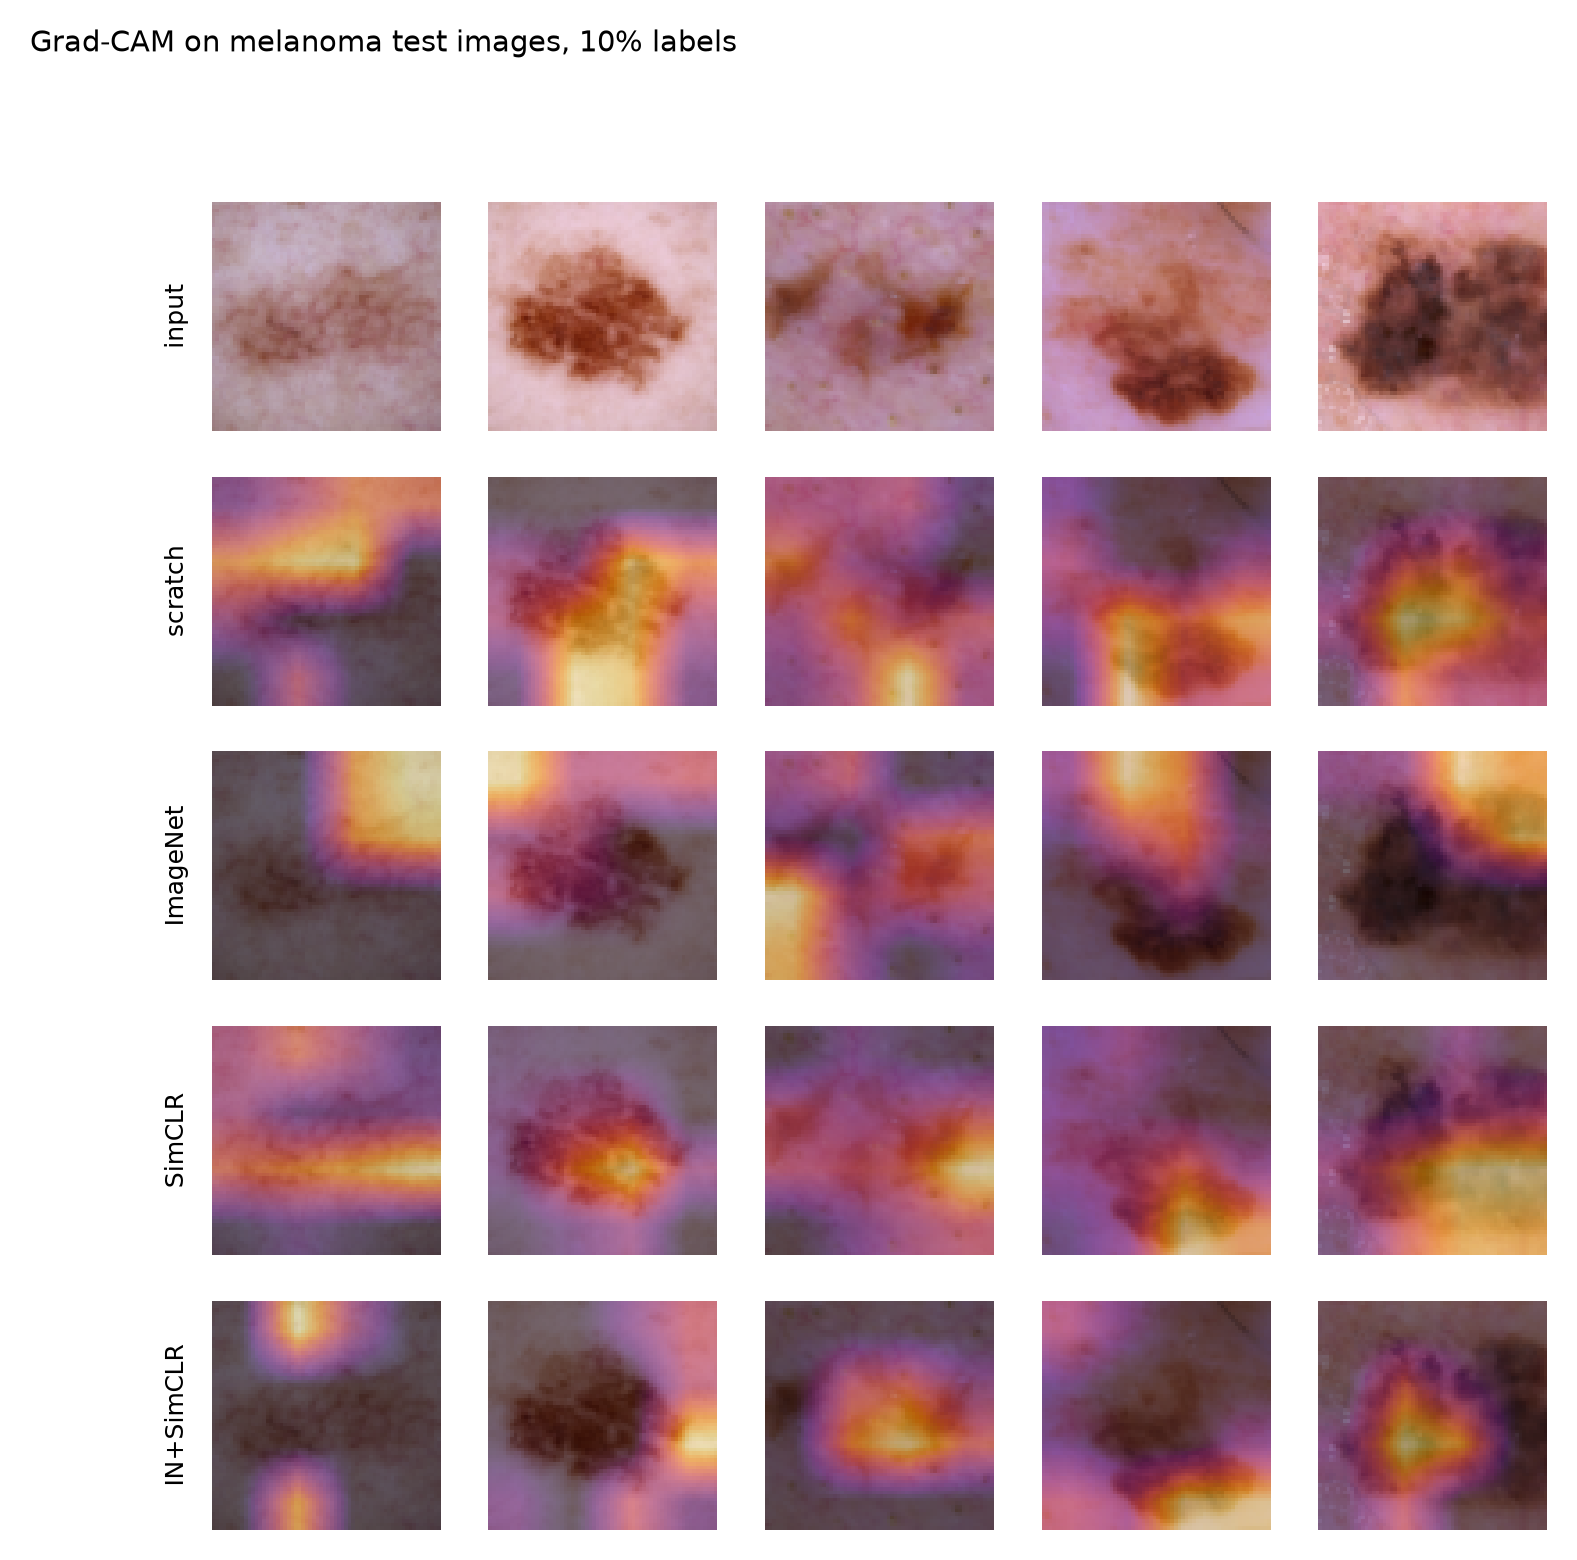
\includegraphics[width=0.72\textwidth]{figs/fig5_gradcam.png}
\caption{Grad-CAM for melanoma test images at the 10\% label budget. Attributions are
coarse at this input resolution and frequently emphasise tissue surrounding the lesion
for every initialisation, so we draw no interpretability advantage from pretraining.}
\label{fig:gradcam}
\end{figure}

\paragraph{Threats to validity.} Three seeds give wide intervals, so the dermatoscopy
ImageNet gains ($+0.028$ at 10\%, $p=0.18$) are directional rather than established, and
only the X-ray SimCLR effects clear $p<0.05$. Resolution is fixed at $64\times64$, which
limits both absolute performance and attribution quality. The unlabelled corpus is small
(fewer than 7{,}000 images), which likely understates what in-domain self-supervision can
achieve on dermatoscopy. Hyperparameters were set once per arm type from standard practice
rather than tuned per cell, a deliberate trade of peak numbers for comparability.
Assumption diagnostics for the paired tests were not assessed.

\section{Conclusion}

Holding everything but the initialisation fixed across 210 supervised runs on two
modalities, we find that the choice between in-domain self-supervision and ImageNet
transfer is not a matter of which method is better but of how far the target modality sits
from natural images. On grayscale chest radiography, SimCLR pretraining on fewer than
5{,}000 unlabelled in-domain images delivers $+0.042$ AUROC over random initialisation at
a 47-image label budget and yields a representation that is linearly decodable
($0.989$ AUROC from a frozen backbone), while ImageNet transfer provides no significant
benefit at any budget. On RGB dermatoscopy the conclusion reverses. The augmentation
ablation supplies a mechanism: colour jitter, standard in SimCLR, must be removed for
dermatoscopy, where colour is diagnostic, and retained for radiography, where it acts as
intensity augmentation. Pretraining advantages vanish at full supervision, in-domain
SimCLR is the best-calibrated and most corruption-robust arm, and no strategy rescues
classes with fewer than a hundred examples.

What we take from the project is that the informative experiments were the ones designed
so that a hypothesis could fail visibly in either direction, and that the results most
worth reporting --- the inverted colour-jitter effect and the off-distribution collapse of
the composed arm --- were ones no accuracy table would have surfaced. Natural extensions
are a larger unlabelled corpus and higher resolution for dermatoscopy, text-supervised
pretraining where reports exist \citep{zhang2022convirt,huang2021gloria}, and a
quantitative measure of domain distance that could predict the inversion point before any
pretraining is run.

\section*{Reproducibility and code}

All code, result tables and figures accompany this report. The pipeline is
\texttt{run\_pretrain.py} (SimCLR checkpoints), \texttt{run\_sweep.py} (label-budget
grid), \texttt{run\_baselines.py}, \texttt{run\_ablation.py}, \texttt{run\_robustness.py},
\texttt{run\_gradcam.py} and \texttt{make\_figures.py}; shared code is in \texttt{src/}.
Seeds $\{0,1,2\}$ control initialisation, label subsampling and augmentation sampling.
Model and training code is written against PyTorch and torchvision
\citep{he2016resnet}; batched GPU augmentation uses Kornia \citep{riquelme2025kornia};
SimCLR follows \citet{chen2020simclr} and Grad-CAM follows \citet{selvaraju2017gradcam};
no third-party implementation was copied. Generative AI (Claude) was used for code
scaffolding, debugging and draft text as described in Section~4; all experimental design
decisions, validity checks and result interpretations are the authors'.

\bibliography{refs}

\end{document}
